\subsection{Spectroscopy Exposure Times} % (fold)
\label{sub:calculation_of_exposure_times}
	The method of calculation for spectroscopic exposure times is much the same as for photometry discussed previously. However, light from the galaxies will not fall in one place on the CCD; instead it will be dispersed by the grating or prism in the spectrometer device. Therefore, it is not possible to use the same equation to determine $N_\text{pix}$ as has been done previously. In order to calculate $N_\text{pix}$ for spectroscopy, the spectral resolution of the dispersive medium being used must first be considered. This can be found using the relationship
	\begin{align}
		R &= \frac{\lambda}{\Delta\lambda}
	\end{align}
	Where $R$ is the resolving power of the diffraction grating or prism and $\lambda$ is the red-shifted wavelength of the Lyman-$\alpha$ absorption line. If these are both known then, $\Delta\lambda$ the spectral resolution can be found for the diffraction grating or prism being used. This is put in place of the band width used in photometry. Light will fall on the CCD in a narrow strip across its width. For the purposes of simplicity, this report will assume that light falls across the entire width of the CCD. This is shown in Figure~\ref{fig:multi_object_spectrum}.
	\begin{figure}[htbp]
		\centering
		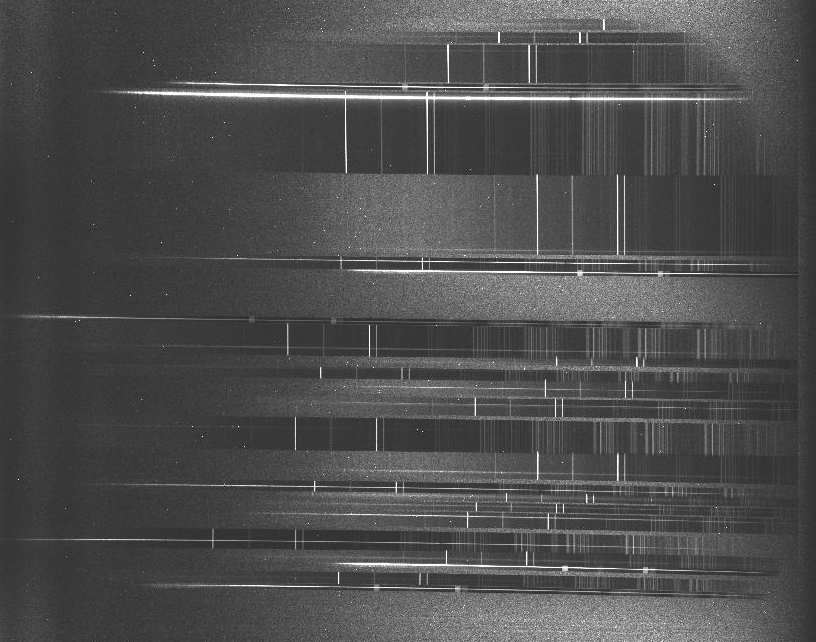
\includegraphics[width=0.5\textwidth]{../Images/Multi_Object_spectrum_picture.png}
		\caption{Photograph of HST orbiting the Earth.\label{fig:multi_object_spectrum}}
	\end{figure}

	The wavelength range this corresponds to is just the wavelength range that can be dispersed particular to the grating or prism being used. The number of pixels across the width of the CCD is known, therefore the wavelength range to which each pixel corresponds can be found. Hence, the number of pixels the spectral resolution can also be found. This value is then multiplied by the spatial resolution element, the number of pixels on the CCD to which the galaxy subtends, to give $N_\text{pix}$. The spatial resolution element has been found to be in the order of a few for the size and redshifts of galaxies considered\cite{SpatialRes}.

	Background for the JWST will mainly be from zodiacal light and thermal radiation from the sun. However, like the flux from the galaxies being observed it will be dispersed by the prism or grating in the spectrometer. Therefore, to calculate the total sky background, the background per pixel is multiplied by the number of pixels in each spectral resolution element.

	In order to estimate the exposure times more accurately the width the spectrums cover the CCD must be known. For a given distance between the dispersive medium and CCD this can be found, but as the spectroscopic devices for the JWST and E-ELT are still undergoing development this distance is unknown. When using NIRSpec's multi-shutter array for multi-object spectroscopy, the widths of the spectrums will depend where the galaxies fall within the field of view, and will not necessarily fit across the entire width of the CCD.

	However, both the JWST and the E-ELT have been designed to optimise the space on the CCD to achieve a maximum resolution. The estimates of exposure times will be upper limits as the calculations are integrated over the maximum number of pixels possible by using the full width of the CCD. Table~\ref{tab:exporure_times_telescops} shows the exposure times for both the JWST and the E-ELT for a selection of high red shift galaxy targets.
	\begin{table}[htbp]
		\begin{center}
			\begin{tabular}{c|c|c}
				\multirow{2}{*}{$M_AB$, $z$} & JWST NIRSpec & E-ELT HARMONI  \\
				 & (Prism $R=100$) & (H+K $R=3900$) \\
				\hline\hline
				30, 8.5 & \SI{4.39e4}{\second}  & \SI{3.31e5}{\second} \\
				29.5, 10 & \SI{6.82e4}{\second} & \SI{1.54e5}{\second} \\
				30.5, 15 & \SI{5.54e5}{\second} & \SI{1.38e6}{\second}
			\end{tabular}
		\end{center}
		\caption{Exposure times for two telescopes for different redshifts.\label{tab:exporure_times_telescops}}
	\end{table}

	A method for more accurate calculation of exposure times is given below providing all relevant information regarding the spectrographs is known, it is a slight variation on the method used for photometry
	\begin{align}
		C &= \frac{I_\lambda N_{\lambda \text{spix}}S_\lambda^d N_{\lambda \text{spix}}}{G}
	\end{align}
	where
	\begin{itemize}
		\item $C =$ Counts per pixel from astronomical source,
		\item $S =$ Instrument spectral sensitivity,
		\item $G =$ Gain (This is the conversion from electrons to ADUs),
		\item $I =$ Flux from the astronomical source,
		\item $N_{\lambda \text{spix}} =$ Number of pixels in the spatial direction,
		\item $N_{\lambda \text{spix}} =$ Number of pixels in the spectral direction.
	\end{itemize}
	Having found the Counts we can then use equation~\ref{eq:Counts}\cite{Counts} to find the time required for a desired signal to noise ratio
	\begin{align}
		\frac{S}{N} &= \frac{CtG}{\sqrt{CtG + N_\text{pix}(B_\text{sky} + B_\text{det}) Gt + \frac{N_\text{pix}}{N_\text{bin}}(N_\text{read} R^2)}} \label{eq:Counts}
	\end{align}
	where
	\begin{itemize}
		\item $t =$ Exposure time (s),
		\item $N_\text{pix} =$ Number of pixels integrated over,
		\item $B_\text{sky} =$ Sky background (photons/sec/pixel),
		\item $N_\text{bin} =$ Total number of binned pixels on CCD,
		\item $N_\text{read} =$ Number of CCD readouts,
		\item $R =$ Read noise (electrons)\cite{}[18]\cite{}[19].
	\end{itemize}
% subsection calculation_of_exposure_times (end)
